\documentclass[letterpaper,11pt]{article}
\usepackage[spanish]{babel}
\usepackage{graphicx}
\usepackage{url}
\usepackage[utf8]{inputenc}
\usepackage{listings}
\usepackage{longtable}
\usepackage[small,bf]{caption}
\setlength{\parindent}{1em}

\begin{document}

\begin{figure}[htp]
  \centering
  
\includegraphics[scale=0.1]{logoUSB.png}
\end{figure}

\begin{center}
  \textbf{UNIVERSIDAD SIM\'ON BOL\'IVAR}\\
  Ingenier\'ia de la Computaci\'on\\
  Dise\~no de Algoritmos I - CI-5651
\end{center}
\begin{center}	
  \vspace{2in}
  \textsf{\begin{Large}\bf Implementaci\'on de un SAT-Solver para la resoluci\'on 
de instancias SAT de sudoku\end{Large}}

\begin{Large}
2da. Entrega
\end{Large}
      
\end{center}
\begin{center}
  \vspace{2in}
Grupo 4\\ 
Federico Flaviani 99-31744\\
Juan Garc\'ia 05-38207\\
  \vspace{0.25in}	
  \today
\end{center}
\newpage

\tableofcontents

\newpage
\setlength{\parskip}{8pt}. 
\section{Introducci\'on}
\emph{Sudoku} es un juego originario de Jap\'on que tiene como objetivo 
rellenar una cuadr\'icula de 9 x 9 celdas (81 casillas) divid\'ida en 
subcuadr\'iculas de 3 x 3 (tambi\'en llamadas ``cajas'' o ``regiones'') 
con las cifras del 1 al 9 partiendo de algunos n\'umeros ya dispuestos 
en algunas de las celdas. La idea es que no se debe repetir ninguna cifra en una 
misma fila, columna o subcuadr\'icula. Un sudoku est\'a bien planteado si la 
soluci\'on es \'unica.
\begin{figure}[htp]
  \centering
  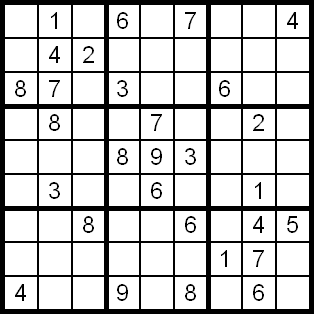
\includegraphics[scale=0.3]{sudoku.png}
  \caption{Ejemplo de un tablero de \emph{Sudoku}}
\end{figure}\\
El objetivo del trabajo que se desarrollara es usar los recursos y herramientas computacionales
para hallar una soluci\'on al juego del sudoku de una manera r\'apida y eficiente.
\subsection{Motivaci\'on del proyecto}
A partir del an\'alisis de complejidad de algunos algoritmos, espec\'ificamente de 
aquellos que entran en el cunjunto de los NP (Nondeterministic Polynomial time), 
nos encontramos con el problema del sudoku general, un problema categorizado como 
NP-Hard, en donde hallar una soluci\'on se resume a realizar busquedas profundas 
dentro del ambiente de estados posibles.

La idea general es aplicar nuevos m\'etodos que 
permitan hallar la soluci\'on de una manera mas eficiente. Hasta ahora hemos aplicado el 
m\'etodo simple que es usar \emph{Backtracking}, en donde vamos asignando variables verificando
estados con soluciones parciales. Adem\'as le agregamos dos t\'ecnicas que ayudan a podar un poco
el \'arbol de estados que se va generando, Pure Literal Elimination en primer lugar y despu\'es
Unit Propagation. Esto hace que el algoritmo sea mas r\'apido en encontrar la soluci\'on.

Ahora la motivaci\'on se centra en querer bajar aun mas esos tiempos y lograr un rendimiento
parecido a solvers como Zchaff, y para ello intentaremos implementar la t\'ecnica de \emph{Backtraking no cronol\'ogico} 
usando \'arboles de asignaciones e incidencias.

\subsection{Breve descripci\'on del problema}
Dada una instancia de Sudoku con solo asignaciones parciales, se plantea buscar 
una soluci\'on, o lo que es igual, hallar el conjunto de asignaciones que deban 
realizarse para rellenar el tablero, y que satisfagan las condiciones de sudoku. 
Estas condiciones son las siguientes:
\begin{description}
\item[-] Cada celda debe contener un n\'umero del 1 al 9.
\item[-] Una celda no puede tener dos n\'umeros distintos.
\item[-] Dos casillas distintas en una misma fila, columna o subcuadr\'icula no 
puede contener el mismo n\'umero.
\end{description}

Para representar estas condiciones usaremos la \emph{Forma Normal Conjuntiva (CNF)}, 
en donde la f\'ormula del problema se plantea como una conjunci\'on de disjunciones, 
y el objetivo es encontrar el conjunto de asignaciones a las variables que mantengan
la condici\'on de \emph{True} en la f\'ormula.

Una f\'ormula CNF consta de una una serie de cl\'ausulas $C_1, C_2, ..., C_n$ agrupadas en una
conjuncion $C_1 \wedge C_2 \wedge ... \wedge C_n$, donde cada cl\'ausula es una disjuncion de
literales $x_1 \vee x_2 \vee ... \vee x_n$ y cada literal representa una variable booleana $X_i$
que puede tomar valores negados $\overline{x_i}$ o no negados $x_i$. Entonces un ejemplo de una 
formula en CNF es la siguiente: $$ (x_1 \vee x_2 \vee x_4) \wedge (\overline{x_3} \vee \overline{x_5}) \wedge (x_7 \vee \overline{x_8} \vee x_9)$$

El objetivo es encontrar asignaciones a las variables $X_i$ tal que la formula siempre sea \emph{True}, y
entonces al asignar todas la variables, esa sera una solucion al problema. En cambio
si para toda asignacion posible encontramos que la formula siempre es \emph{False}, el problema
no tiene solucion.

\subsection{Descripci\'on del contenido del informe}
En el siguiente informe se dar\'a una breve explicaci\'on del dise\~no e 
implementaci\'on del sat-solver orientado a la resoluci\'on del sudoku. Basicamente 
se explicar\'an las estructuras de datos usadas para representar el problema y los 
algoritmos utilizados. Adem\'as presentar aquellos problemas encontrados durante el 
desarrollo, una breve rese\~na de los elementos implementados y detalles en cuanto 
a la operatividad del programa. En general estamos presentando una guia para 
entender la manera en que atacamos la idea y como generamos una soluci\'on razonable 
para el problema del Sudoku.
\newpage

\section{Dise\~no}

\subsection{Modelo utilizado para representar el problema}
El modelo general para la resoluci\'on del problema del \emph{Sudoku} se basa en
tres partes. Un proceso de traducci\'on del problema a representaci\'on
SAT, siguiendo las restricciones las reglas de resoluci\'on del juego. Luego la
busqueda de la soluci\'on mediante el sat-solver, el cual recibe la traducci\'on antes
realizada. Por \'ultimo tomar la salida del solver y convertirla en una soluci\'on sudoku
mas legible. Por lo tanto nuestra implementaci\'on tendra 4 m\'odulos, donde se destacan, un m\'odulo de \emph{Traducci\'on} 
del problema, uno de \emph{Herramientas auxiliares} a usar en el algoritmo del solver, otro m\'odulo
que implementa directamente los algoritmos que llamaremos \emph{Solver} y por \'ultimo uno de gerencia que
permitira correr las diferentes instancias con una sola ejecuci\'on, a este lo llamaremos el m\'odulo de \emph{Soluci\'on}.

La representaci\'on SAT se realiz\'o usando la forma normal conjuntiva (CNF) mencionada anteriormente, en donde
cada cl\'ausula que restringe el problema es presentada como una disjuncion de literales, 
y la f\'ormula total es una conjunci\'on de cl\'ausulas. Los literales no son mas que asignaciones 
\emph{True} o \emph{False} de variables en forma positiva (i) o negativa (-i). Fueron implementadas una serie
de estructuras para representar a nivel computacional la f\'ormula CNF, una clausula y un literal, pero
adelante se daran mas detalles al respecto.

Se utiliz\'o la representaci\'on de un \'arbol de estados, en donde cada nodo es una f\'ormula CNF
con una asignaci\'on que es soluci\'on parcial del problema. Una soluci\'on parcial del problema es cuando todas las
cl\'ausulas del problema se encuentran no asignadas totalmente o ya est\'an satisfechas. En caso de que exista una
cl\'ausula no satisfecha ya no es soluci\'on parcial. La idea es ir generando sucesores para recorrer
el \'arbol y buscar una soluci\'on al problema donde todas las clausulas sean satisfechas.

Un sucesor de un nodo del \'arbol es aquella f\'ormula generada a partir de una asignaci\'on hecha a una variable,
y que sigue siendo una soluci\'on parcial. Por lo tanto se generar\'a un arbol binario, ya que solo existen dos posibles sucesores,
cuando le asignes \emph{True} o \emph{False} a una variable. Es posible generar un sucesor despu\'es de hacer
varias asignaciones, en este caso hablamos de aplicar Pure Literal Elimination o Unit Propagation para hacer varias
asignaciones en cascada siguiendo una serie de criterios, y esto siempre con valores \emph{True}. Al final una hoja del \'arbol 
sera una f\'ormula CNF con todas las variables asignadas, siendo esta soluci\'on o no.

\subsection{ Estructuras y algoritmos involucrados en la aplicaci\'on}
A continuaci\'on se explicaran las estruturas y algoritmos utilizados, lo dividiremos en
diferentes secciones, segun los m\'odulos explicados anteriormente:

\subsubsection{Traducci\'on}
El m\'odulo de traducci\'on se basa en leer las instancias parciales de sudoku, para luego 
mediante cl\'ausulas en CNF representar el problema general en formato SAT-DIMACS,
todo esto en conjunto con las asignaciones parciales realizadas. Todos los algoritmos utilizados
fueron simples iteraciones que iban escribiendo en el archivo de salida (``out.cnf''), las
cl\'ausulas necesarias segun las restricciones del problema.

\subsubsection{Herramientas Auxiliares}
En este m\'odulo destaca la creaci\'on de una lista simple enlazada, que sera la estrucutura
que nos permitir\'a llevar un registro de literales y cl\'ausulas de una f\'ormula en CNF. B\'asicamente
se implement\'o el tipo abstracto \emph{List} junto con una serie de operaciones elementales que trabajan
sobre el tipo para agregar, eliminar y recorrer elementos de la misma.

\subsubsection{SAT-Solver}
Para el SAT-solver fue necesario crear una serie de estructuras para representar de manera general
una f\'ormula normal conjuntiva. Se cre\'o un arreglo para almacenar cada uno de los literales en memoria, y
los mismos se guardan en una estructura con diferentes campos, espec\'ificamente un 
campo que guarda el valor asignado y una lista de cl\'ausulas asociadas al literal.
Para representar una cl\'ausula se crea una estrucutra que guarda contadores sobre
los literales satisfechos o no satisfechos, asi como el tama\~no de una cl\'ausula,
una lista de literales que la componen y un literal que resguarda cuando una cl\'ausula es unitaria.
Para generalizar la f\'ormula, se crea una estructura que representa una f\'ormula
conjuntiva  y guarda el n\'umero de literales y cl\'ausulas totales, el arreglo de
literales, el n\'umero de cl\'ausulas satisfechas y las variables asignadas.

En la versi\'on que implementamos del algoritmo DPLL, lo primero que se realiza
es la verificaci\'on de que la f\'ormula de entrada es soluci\'on o no. De ser soluci\'on se retorna
un valor True, si no, se procede con el grueso de la funci\'on.
Primero se aplica Pure Literal Elimination, en donde aquellos literales que no tengan
cl\'ausulas asociadas induciran un valor de True en el valor opuesto de dicho literal.
Luego se procede a elegir el primer literal a asignar, si no existe ning\'un literal para
seleccionar y no existe soluci\'on, pues se retorna False, y en caso que todas las variables hayan sido
asignadas y se encuentra soluci\'on, el algoritmo termina entregando la respuesta buscada. En caso de que aun
existan variables por asignar, se hace la asignaci\'on de esta nueva variable y 
se ejecuta Unit Propagation. Unit Propagation se encargar\'a de buscar esas cl\'ausulas unitarias en donde se
puedan asignar True al literal unitario y satisfacer la cl\'ausula, de esta manera se hacen asignaciones cascada
que pueden disminuir el tiempo de busqueda. Luego basta con llamar recursivamente DPLL con la nueva f\'ormula generada, 
si esta llamada recursiva retorna False se procede a restaurar las asignaciones hechas en el Unit Propagation y se hace
backtracking para asignar el otro valor a la variable primeramente asignada. 

La esencia del DPLL es ir asignando variables, y mientras se vayan generando cl\'ausulas unitarias
aplicar Unit Propagation. Y ahora gracias al backtracking no cronol\'ogico vamos a poder regresarnos a niveles
superiores al inmediato anterior, y asi realizar una mejor poda del \'arbol de posibles soluciones.

Para realizar un backtracking no cronol\'ogico es necesario ir generando en 
el momento de las asignaciones un grafo de implicaciones, que ser\'a 
destruido en el momento del backtracking. Los nodos de este grafo son 
asignaciones del tipo $x_i  valor, nivel, desicion)$, donde $valor$ es el 
valor de verdad de la variable $x_i$, $nivel$ es el nivel donde fu\'e 
asignada la variable y $desicion$ es un booleano que determina si la 
asignaci\'on fu\'e de desici'on o implicada por otras asignaciones, ademas 
existe un nodo adicional llamado $\kappa$ que simboliza un conflicto. El 
grafo de implicaci\'on, es un grafo dirigido donde $(a,b)$ es una arista 
si y s\'olo si la asignaci\'on $b$ es implicada por $a$.

Una vez que el grafo de implicaciones llega a un conflicto, se procede a buscar todas las asignaciones de desici\'on, que son alcanzables desde 
$\kappa$ en el grafo de implicaci\'on anterior pero con el sentido de las aristas cambiadas. Para implementar esa busqueda usamos el algoritmo de DFS recursivo. 

La implementaci\'on de un algoritmo de DFS es bastante eficiente cuando se usan listas de adyacencias como estructura de datos que representan nuestro grafo. Sin embargo, el grafo al que se le aplica la busqueda en profundidad, no es el grafo de implicaciones, si no, uno igual salvo el sentido de sus aristas. Por lo tanto, tomamos la desici\'on de implementar el grafo de implicaciones con listas de incidencias, ya que estas mismas listas ser\'ian las listas de adyacencias, del grafo invertido al que se le aplicara la busqueda en profundidad.

\subsubsection{Soluci\'on}
Por \'ultimo tenemos el m\'odulo de soluci\'on, en donde se recibe la salida de los
respectivos solver y se procede a representar la soluci\'on obtenida en formato 
de sudoku general. Luego de esto se genera un archivo en formato Pdf que mostrar\'a la cuadr\'icula
con la soluci\'on de la instancia correspondiente.
\newpage

\section{Detalles de implementaci\'on}

\subsection{Rese\~na de los elementos implementados}
La estructura de datos que implementa la formula proposicional en forma 
normal conjuntiva viene dada por la siguiente estructura:

\subsubsection{Objeto Literal}
La implementaci\'on del objeto literal viene dado por un registro con tres 
campos: $value$, $asig$ y $clauses$. El primero de ellos representa el valor de 
verdad del literal, el segundo un tipo $Asignation$ que se guardara en el \'arbol de asignaciones para el 
bactracking no cronol'ogico y el tercero es una lista de de las cl\'ausulas que contienen 
a dicho literal.

\begin{verbatim}
struct literal {
	  int value;
	  Asignation asig;
	  List clauses;
}
\end{verbatim}

\subsubsection{Objeto Cl\'ausula}
La implementaci\'on del objeto Cl\'ausula viene dado por un registro con 
seis campos: $numSat$, $numNotSat$ son enteros que determinan 
cuantos literales est\'an satisfechos o no en la Cl\'ausula en determinado 
momento, $isSatisf$ nos dice cuando una clausula es satisfecha, $size$ es el tama\~no 
de la clusula, $literals$ es una lista que contienen todos los literales de 
la cl\'ausula y $unitLit$ es un apuntador que se\~nala a un literal, en 
el momento en que para una soluci\'on parcial \'este sea unitario.

\begin{verbatim}
struct clause {
	  int numSat;
	  int numNotSat;
	  int isSatisf;
	  int size;
	  List literals;
	  Literal unitLit;
}
\end{verbatim}

\subsubsection{Objeto F\'ormula}
La implementaci\'on de la F\'ormula viene dada por un registro de 9 campos:
$numLiterals$, $numVar$ y $numClauses$ son tres enteros que matienen el n\'umero total
de literales, n\'umero de variables y el n\'umero de cl\'ausulas. $literals$ y $clauses$ es un arreglo
con todos los literales y una lista con la cl\'ausulas respectivamente. $satClauses$ es el n\'umero de
cl\'ausulas satisfechas, $numVarAssig$ el n\'umero de variables asignadas en un estado dado, $isTrue$
es un booleano que indica si la f\'omula esta satisfecha y $assigUnitProp$ es una lista de literales
asignados en una llamada a Unit Propagation.

\begin{verbatim}
struct form {
	  int numLiterals;
	  int numVar;
	  int numClauses;
	  Literal *literals;
	  List clauses;
	  int satClauses;
	  int numVarAssig;
	  int isTrue;
	  List assigUnitProp;
}
\end{verbatim}

En el arreglo de literales colocamos los $2*|Var|$ posibles literales 
que existen sobre un conjunto de variables $Var$, en las posiciones 
dadas por la siguiente formula. 

$$literales[j]=\left\{\begin{array}{lcc}
              x_{(j/2)+1} & si & j~es~par \\
             \\ \overline{x_{(j+1)/2}}   & si & j~es~impar
             \end{array}
      \right.  $$

De esta forma $j$ identifica univocamente a cada literal, y por lo tanto 
basta saber el \'indice de alg\'un literal en particular, para ubicarlo dentro 
de una casilla del arreglo $literales$.

\subsubsection{Objeto Asignaci\'on}
Son las estructuras que representan una asignacion en nuestro \'arbol de asignaciones.

\begin{verbatim}
struct asignation {
	  int desition;
	  int variable;
	  int value;
	  int level;
}
\end{verbatim}

\begin{verbatim}
struct asignationTree {
	  List incidents;
	  List leaf;
	  Asignation asigMaxLevel;
}
\end{verbatim}

\begin{verbatim}
struct treeVertice {
	  Asignation asig;
	  List incident;
}
\end{verbatim}

\subsection{Problemas encontrados}
\begin{itemize}
\item La estructura de datos que usamos nos permite saber si una cl\'ausula 
es unitaria f\'acilmente. Sin embargo, no podemos saber con costo constante 
cual es el literal unitario de cada cl\'ausula unitaria, ya que tendriamos que 
recorrer toda la lista de literales para saberlo.
\item La implementaci\'on de la lista utilizada para almacenar elementos nos genera
una serie de memory leaks al momento de agregar un elemento. Esto debido a que la definici\'on
recursiva utilizada no soporta el inmenso overhead que se genera al reservar memoria
rapidamente en cortos periodos de tiempo. Por lo tanto para instancias que tarden un tiempo
considerable en ser resueltas, esto puede representar un problema a nivel de exceso de memoria
utilizada.
\end{itemize}
\newpage

\section{Instrucciones de operaci\'on}
Para la ejecuci\'on del programa se tienen dos opciones, correr un script en Python
que permite realizar todas las corridas de las instancias dadas en clase, o correr
por separado el traductor con alguna instancia en un formato determinado y luego el
solver con el archivo en CNF de un problema en SAT.

\subsection{Script en Python}
La aplicaci\'on en Python llama al compilador para 
generar los distintos ejecutables, luego procede a corre el traductor para
representar la instancia dada en formato SAT, y luego llamar a los respectivos
solvers para la resoluci\'on del problema. Al obtener la soluci\'on, procede a
generar los respectivos archivos en .pdf.

Con respecto a paquetes o librerias especiales en caso que quiera correr el script
se necesita lo siguiente:
\begin{description}
\item[-] Compilador Gcc para los programas escritos en C
\item[-] Libreria para correr programas en Python
\item[-] Libreria PdfLatex para generar los tableros
\end{description}
Y la \'unica linea que debera correr es la siguiente:
\begin{verbatim}
    $> python satSolver.py
\end{verbatim}

\subsection{Traductor y Solver}
Como se mencion\'o anteriormente se puede compilar y correr por separados el traductor y el solver.
Simplemente es necesario tener instalado un compilardor de C, recomdamos el antes mecionado Gcc.

Para compilar los diferentes programas se debe usar el comando: 
\begin{verbatim}
    $> make
\end{verbatim}

Para compilar el traductor por separado solo debe realizar la llamada:
\begin{verbatim}
    $> make translator
\end{verbatim}
Y para realizar la corrida:
\begin{verbatim}
    $> ./translator N_InstanciaParcial out.cnf
\end{verbatim}
El segundo argumento es una isntancia parcial del sudoku, en donde el primer 
numero N es el tama\~no del sudoku, luego un underscore (\_) y seguido la Instancia con
asignaci\'on parcial al estilo de las entregadas en clase del archivo ``InstanciasSudoku.txt''. 
La traduccion a SAT se entrega en el archivo ``out.cnf''

Luego para compilar el solver debe llamar:
\begin{verbatim}
    $> make solver
\end{verbatim}
Y para correr el programa:
\begin{verbatim}
    $> ./solver out.cnf
\end{verbatim}
Donde out.cnf es la traducci\'on del problema de Sudoku a SAT.

Para compilar el solver de ZChaff:
\begin{verbatim}
    $> cd zchaff64/
    /zchaff64 $> make 
\end{verbatim}
Y debe correrse con la llamada a:
\begin{verbatim}
    $> ./zchaff64/zchaff out.cnf
\end{verbatim}
\newpage

\section{Estado actual}

\subsection{Estado final de la aplicaci\'on}
El estado final de la aplicaci\'on no es operativo al 100\%, espec\'ificamente en el m\'odulo del solver.
El traductor realiza su funci\'on perfectamente, tomando del archivo las instancias de sudoku
y entregando la traducci\'on a CNF. De igual manera el m\'odulo de soluci\'on, en donde se toma
la salida de los solvers y se entrega en formato sudoku pdf tambi\'en funciona.
\subsection{Errores}
Aunque fue resuelta la problem\'atica con el algortitmo de DPLL, tenemos algunos memory leaks que hacen que
para instancias que tardan mucho tiempo, el consumo de memoria sea muy grande, pudiendo llegar a veces a
dejar sin memoria al equipo y entonces el sistema operativo manda una se\~nal de kill al proceso. Para instancias
que duran poco tiempo, aproximadamente menos de 20 min, corre perfecto y encuentra la soluci\'on.

Otro problema es que no se logro implementar el arbol de asignaciones de manera correcta, por lo tanto el grafo
generado no representa la estructura ideal para realziar un backtracking a mayores niveles. Son problemas en la
elecci\'on del literal a asignar, que esta creando ciclos en el grafo, lo que genera una problem\'atica al momento de
buscar una soluci\'on.

\newpage

\section{Conclusiones y recomendaciones}
Dado que no fue posible cumplir los objetivos planteados en el problema, son pocas las conclusiones
que podemos sacar. En general encontramos una serie de problemas para implementar una buena soluci\'on al problema, mas que todo
por el enfoque que dimos a nivel de programaci\'on de los algoritmos. Por lo tanto resulta de vital importancia
plantear una soluci\'on mas eficiente y concisa de las funciones que se vayan a implementar para desarrollar
el solver.
Aunque no fue posible implementar la solucion optima usando backtracking no cronol\'ogico, se notaron cambios
considerables en los tiempos de corrida al resolver el problema, pasando de minutos a pocos segundos. Esto
demuestra que la tecnica aplicada realiza una poda significativa en el arbol de estados.
\subsection{Resultados obtenidos}
A continuaci\'on se presentan los tiempos de las corridas del solver hecho en el proyecto y el solver Zchaff sobre 
las instancias dadas en el archivo ``InstanciasSudoku.txt''
\begin{center}
\begin{longtable}{|c|c|c|}
\hline
Instancia & Solver propio & Solver Zchaff\\
\hline
1 & 225.671 ms & 0.00786 ms \\
\hline
2 & $\geq$ 5 min & 0.00381 ms \\
\hline 
3 & $\geq$ 5 min & 0.00405 ms \\
\hline
4 & 80.051 ms & 0.00691 ms \\
\hline
5 & 14872.498 ms & 0.00786 ms \\
\hline
6 & 29.879 ms & 0.00715 ms \\
\hline
7 & 816.949 ms & 0.00691 ms \\
\hline
8 & 135.041 ms & 0.00715 ms \\
\hline
9 & 167.229 ms & 0.00786 ms \\
\hline
10 & 125827.757 ms & 0.00810 ms \\
\hline
11 & 2371.787 ms & 0.00691 ms \\
\hline
12 & 2416.908 ms & 0.0128 ms \\
\hline
13 & 547.145 ms & 0.00715 ms \\
\hline
14 & 56456.277 ms & 0.00786 ms \\
\hline
15 & $\geq$ 5 min & 0.00381 ms \\
\hline
16 & 137.175 ms & 0.00691 ms \\
\hline
17 & 90.197 ms & 0.00691 ms \\
\hline
18 & $\geq$ 5 min & 0.00405 ms \\
\hline
19 & 71.579 ms & 0.00715 ms \\
\hline
20 & 46656.309 ms & 0.00810 ms \\
\hline
21 & 54.132 ms & 0.00905 ms \\
\hline
22 & 239.806 ms & 0.00786 ms \\
\hline
23 & 7772.205 ms & 0.00691 ms \\
\hline
24 & 185214.636 ms & 0.00691 ms \\
\hline
25 & $\geq$ 5 min & 0.00286 ms \\
\hline
26 & $\geq$ 5 min & 0.00309 ms \\
\hline
27 & $\geq$ 5 min & 0.00405 ms \\
\hline
28 & 144028.009 ms & 0.00715 ms \\
\hline
29 & 428.553 ms & 0.00691 ms \\
\hline
30 & 2008.273 ms & 0.00786 ms \\
\hline
31 & 391.221 ms & 0.00691 ms \\
\hline
32 & 5074.174 ms & 0.00715 ms \\
\hline
33 & $\geq$ 5 min & 0.00309 ms \\
\hline
34 & 144701.276 ms & 0.00786 ms \\
\hline
35 & $\geq$ 5 min & 0.00405 ms \\
\hline
36 & $\geq$ 5 min & 0.00381 ms \\
\hline
37 &  1203.404 ms & 0.00810 ms \\
\hline
38 & 20366.432 ms & 0.00715 ms \\
\hline
39 & 50972.270 ms & 0.00691 ms \\
\hline
40 & 395472.976 ms & 0.00715 ms \\
\hline 
41 & 146.774 ms & 0.00691 ms \\
\hline
42 & 158.635 ms & 0.00691 ms \\
\hline
43 & $\geq$ 5 min & 0.00286 ms \\
\hline
44 & 17252.228 ms & 0.00715 ms \\
\hline
45 & 524.287 ms & 0.00715 ms \\
\hline
46 & 383.146 ms & 0.00715 ms \\
\hline
47 & 169821.164 ms & 0.00691 ms \\
\hline
48 & 940.442 ms & 0.00715 ms \\
\hline
49 & 674.192 ms & 0.00786 ms \\
\hline
50 & 172.515 ms & 0.00691 ms \\
\hline
51 & 57.373 ms & 0.00786 ms \\
\hline
52 & 84.462 ms & 0.00786 ms \\ 
\hline
53 & 294.802 ms & 0.00810 ms \\
\hline
54 & 77.813 ms & 0.00691 ms \\
\hline
55 & 163.821 ms & 0.00715 ms \\
\hline
56 & 909.723 ms & 0.00810 ms \\
\hline
57 & $\geq$ 5 min & 0.00309 ms \\
\hline
58 & 84.602 ms & 0.00786  ms \\
\hline
59 & 46.894 ms & 0.00786 ms \\
\hline
60 & 551.743 ms & 0.00786 ms \\
\hline

\end{longtable}
\end{center}
\subsection{Mejoras}
\begin{itemize}
\item Debemos implementar una estructura de lista m\'as eficiente con relaci\'on a la memoria usada, porque
dado el overhead de reservar mucha memoria en poco tiempo, cuando el programa tarda demasiado
la memoria usada crece demasiado.
\item Realizar una mejora en el Backtracking no cronol\'ogico y modificar el metodo que agrega la clausula de
aprendizaje para que lo haga mas eficiente.
\end{itemize}

\newpage

\section{Referencias bibliogr\'aficas}
\begin{thebibliography}{99}
  
\bibitem[1]{ref:data struct}
  \textbf{Efficient Data Structures for Fast SAT Solvers}\\
  \textit{LYNCE I., MARQUES-SILVA J.}

\bibitem[2]{ref:sat format}
  \textbf{Satisfiability Suggested Format}\\

\bibitem[3]{ref:sudoku as sat}
  \textbf{Sudoku as SAT Problem}\\
  \textit{LYNCE I., OUAKNINE J.}

\bibitem[4]{ref:ins sat}
  \textbf{url{http://www.cs.ubc.ca/$~$hoos/SATLIB/Benchmarks/SAT/satformat.ps}}

\bibitem[5]{ref:grasp}
  \textbf{GRASP - A New Search Algorithm for Satisfiability}\\
  \textit{MARQUES SILVA J., SAKALLAH K.}

\bibitem[6]{ref:berkmin}
  \textbf{BerkMin: a Fast and Robust Sat-Solver}\\
  \textit{GOLDBERG E., NOVIKOV Y.}
  
\end{thebibliography}
  
\end{document}
